% Generado por experimentos/analizar_ranking_costo.py (--tag v3_563e683) desde fig_ranking_costo.csv:
% concordancia con el valor de rollout v (pares ordenados como v) de la red y de los mal ubicados, en los niveles de BS+Cost agrupados por
% el costo restante del mejor candidato (sin el tramo 0, en que hay un hijo ya ordenado).
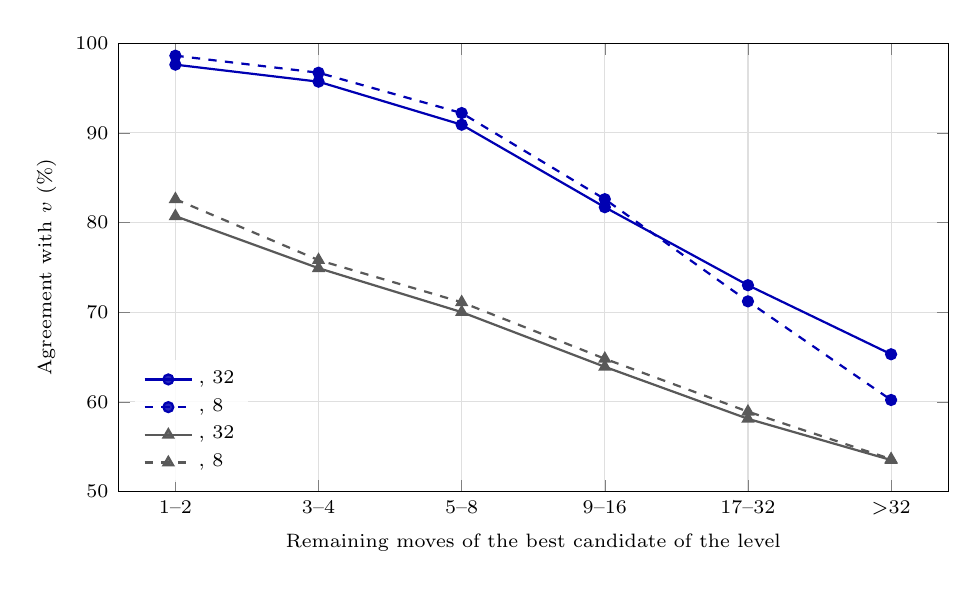
\begin{tikzpicture}
\begin{axis}[
    width=\columnwidth, height=0.6\columnwidth,
    xmin=0.6, xmax=6.4, ymin=50, ymax=100,
    xtick={1,2,3,4,5,6}, xticklabels={1--2, 3--4, 5--8, 9--16, 17--32, ${>}32$},
    xlabel={Remaining moves of the best candidate of the level},
    ylabel={Agreement with $v$ (\%)},
    grid=major, grid style={gray!25},
    tick label style={font=\scriptsize}, label style={font=\scriptsize},
    legend style={font=\scriptsize, at={(0.02,0.02)}, anchor=south west, draw=none, fill=white, fill opacity=0.85, text opacity=1},
    legend cell align=left,
]
\addplot[mark=*, mark size=1.8pt, thick, blue!70!black] coordinates {(1,97.6) (2,95.7) (3,90.9) (4,81.7) (5,73.0) (6,65.3)};
\addlegendentry{$\costhat$, \bw{32}}
\addplot[mark=*, mark size=1.8pt, thick, blue!70!black, dashed, mark options={solid}] coordinates {(1,98.6) (2,96.7) (3,92.2) (4,82.6) (5,71.2) (6,60.2)};
\addlegendentry{$\costhat$, \bw{8}}
\addplot[mark=triangle*, mark size=2.0pt, thick, gray!70!black] coordinates {(1,80.7) (2,74.9) (3,70.0) (4,63.9) (5,58.1) (6,53.5)};
\addlegendentry{$\nbad$, \bw{32}}
\addplot[mark=triangle*, mark size=2.0pt, thick, gray!70!black, dashed, mark options={solid}] coordinates {(1,82.6) (2,75.8) (3,71.1) (4,64.8) (5,58.9) (6,53.6)};
\addlegendentry{$\nbad$, \bw{8}}
\end{axis}
\end{tikzpicture}
